\documentclass[11pt]{article}

\usepackage[margin=1in]{geometry}
\usepackage[T1]{fontenc}
\usepackage[utf8]{inputenc}
\usepackage{newtxtext,newtxmath}
\usepackage{amsmath}
\usepackage{graphicx}
\usepackage{booktabs}
\usepackage{caption}
\usepackage[round,authoryear]{natbib}
\usepackage{setspace}
\usepackage{lineno}
\usepackage[hidelinks]{hyperref}
\usepackage{siunitx}
\usepackage{authblk}

\captionsetup{font=small,labelfont=bf}
\bibliographystyle{apalike}
\graphicspath{{figs/}}
\setlength{\parskip}{0pt}
\linenumbers
\onehalfspacing

\title{\bfseries Keeping the words, losing the thread:\\
word-level coupling survives mind-wandering while comprehension fails where the mind was}

\author[1]{Author One}
\author[1]{Author Two}
\author[2]{Author Three}
\affil[1]{Affiliation}
\affil[2]{Affiliation}
\date{}

\begin{document}
\maketitle

\begin{abstract}
\noindent
Readers often report that their minds have wandered while their eyes kept moving over the page.
The standard explanation is perceptual decoupling. Attention withdraws from the text, so word
properties stop guiding the eyes. That account has been tested almost entirely through one
measure, the duration of a fixation. Reading involves at least three separable decisions about
each word: whether to fixate it, how long to stay, and whether to come back. We tested all
three, together with fixation-locked brain responses, in 44 readers of connected articles
recorded with simultaneous eye tracking and electroencephalography.
The eyes went on doing word-sensitive reading. What failed was what the reader built from the
words.
Word sensitivity was intact throughout mind-wandering. The influence of frequency, length and
contextual surprisal on skipping was statistically equivalent to its on-task value within
$\pm$10\%. Refixation and regression selectivity were preserved. Duration slopes survived a
model that held word identity constant. The occipitotemporal frequency response was preserved to
within 8.2\%. The centroparietal response to contextual surprisal could not be tested usefully
here, so the semantic channel remains open. These measures do register a change when one is
present. An instructed shallow-reading goal in an independent sample attenuated behavioural
coupling by about a third.
The most cited behavioural marker of mindless reading, an increase in skipping, is an artefact
of how skipping is scored in continuous reading. Under a scan-path definition readers skip
18.5\% \emph{fewer} words and work harder on each one.
Comprehension failed even so, and it failed where the mind was rather than where the eyes were.
Accuracy fell from 0.68 with no lapse to 0.41 when a reported lapse covered the sentences
carrying the answer. That effect was more extreme than all of 1000 size-matched regions placed
elsewhere on the same page. The same test run on where the eyes actually went predicted nothing.
Mind-wandering, at least as readers themselves demarcate it, does not disconnect the eyes from
the words. It leaves the words intact and costs the reader what is built from them.
\end{abstract}

\vspace{0.5em}
\noindent\textbf{Keywords:} mind-wandering; reading; eye movements; fixation-related potentials;
perceptual decoupling; equivalence testing

\newpage

\section{Introduction}

Everyone who reads has had the experience of reaching the bottom of a page and realising that
nothing has gone in. The eyes moved, the lines were traversed, and yet no meaning accumulated.
Laboratory work has turned this ordinary failure into a tractable phenomenon: readers probed
during self-paced reading report task-unrelated thought on a sizeable minority of trials, and
those reports are followed by measurable changes in the eye-movement record and in
comprehension \citep{smallwood2006,schooler2011,smallwood2015}.

The standard explanation is perceptual decoupling. On this account attention withdraws from
the external input during mind-wandering, so the products of word identification no longer
reach the systems that program eye movements \citep{smallwood2011cascade,schooler2011}. The
account makes a sharp and testable prediction. If lexical processing is what normally makes
the eyes behave differently for a rare word than for a common one, then the difference should
shrink when the mind is elsewhere. \citet{reichle2010} reported exactly this pattern in a
self-caught paradigm: fixations before self-reported mindless reading were longer and less
sensitive to word frequency and length. \citet{schad2012} showed that the disruption is
graded, with deeper lapses producing larger changes. A recent meta-analysis of eye-movement
markers concluded that the most consistent signatures are an increase in skipping and a
reduction in fixations per word, and that reduced sensitivity to lexical properties is
diagnostic of the deeper form of mindless reading \citep{meziere2025}.

Two features of that evidence base leave the central claim less settled than it appears.

First, the claim is about coupling, and coupling has been measured almost entirely in one
place. Reading is not a single decision. Models that differ in almost every other respect
agree that the eyes make at least three separable choices about each word: whether to fixate
it at all, how long to remain once fixated, and whether to come back
\citep{reichle2003,engbert2005,rayner2009}. These decisions draw on lexical information at
different points and with different latencies. Skipping is decided before the word is
fixated, on parafoveal information, and is strongly driven by length and frequency
\citep{rayner1998,kliegl2004}. Dwell time reflects processing of the fixated word. Regressions
are a repair mechanism deployed after difficulty has been encountered. A withdrawal of
attention that spared one of these and abolished another would look very different from one
that scaled them all (Fig.~\ref{fig:design}b). Fixation duration alone cannot distinguish these
possibilities.

Second, and more practically, fixation duration can only be measured on words that were
fixated. Whether a word is fixated is itself the most lexically driven decision the reader
makes, and it changes during mind-wandering. Conditioning a coupling estimate on a variable
that the manipulation moves is a familiar source of bias. It matters here because the
measurement of skipping in continuous multi-page reading is not straightforward. A word can
fail to receive a fixation because the reader stepped over it in a single saccade, which is
skipping in the sense the models mean, or because gaze and text were transiently out of
register, which is not.

A third gap is neural. Simultaneous eye tracking and electroencephalography now makes it
possible to read out word processing directly, without inferring it from behaviour. Fixation-related
potentials in natural reading carry a graded occipitotemporal response to word frequency
from roughly 150\,ms and a centroparietal N400 that scales with contextual surprisal
\citep{dimigen2011,kutas2011,frank2015}. If mind-wandering gates the input, these responses
should shrink. Almost all co-registered reading work has been conducted on-task, and almost
all mind-wandering reading work has been behavioural. We are not aware of a well-powered test
at the intersection.

We addressed all three gaps in a single design, and then asked what the reader actually loses,
using the page-level comprehension questions that the dataset records.

In the primary dataset, 44 readers read five
connected Wikipedia articles at their own pace while 64-channel electroencephalography and
binocular eye movements were recorded, and reported the spans during which their minds had
wandered. This yielded 404{,}557 first-pass fixations, of which 7.2\% fell inside a reported
span. We measured word sensitivity at all three levels of eye-movement control and in two
fixation-locked neural responses, and we treated the null as something to be supported rather
than merely observed, using equivalence tests and Bayes factors throughout. Because a null is
only as good as the sensitivity of the instrument that produced it, we included a positive
control: an independent sample of 12 readers who read under an instructed shallow-search goal
as well as for comprehension \citep{hollenstein2018}. If our measures can detect a change in
coupling when one is present, then their failure to detect one during mind-wandering is
informative.

What we found is a single dissociation with two halves. During mind-wandering the eyes go on
doing word-sensitive reading: every measure of how strongly word properties govern the reading
system was preserved, in behaviour and in the fixation-locked brain response. What fails is what
is built from those words: comprehension collapses, and it collapses specifically on the
material the reader was absent for, while the record of where the eyes went carries no such
information. The rest of the paper establishes those two halves. It also shows that the same measures do
register a change in coupling when one is genuinely present, and identifies a measurement artefact
that explains part of why the field has read the first half differently.

\begin{figure}[t]
\centering
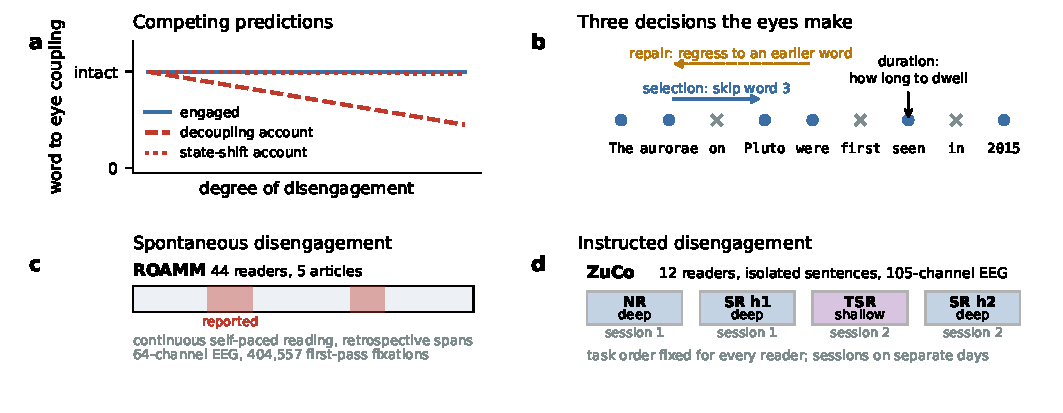
\includegraphics[width=\textwidth]{fig1_design.pdf}
\caption{\textbf{Question and design.}
(a) Perceptual decoupling predicts that the influence of word properties on eye movements
weakens as disengagement deepens; an account in which disengagement is a change of global state
predicts that it does not.
(b) The eyes make at least three separable decisions about each word. Circles mark fixated
words and crosses mark words that were stepped over.
(c) The primary sample. Readers read connected articles at their own pace and afterwards marked
the spans during which their minds had wandered.
(d) The control sample. Readers read isolated sentences under a deep or a shallow goal. Task
order was the same for every reader and the two encyclopedic tasks fell in different sessions,
which we exploit in Section~\ref{sec:goal}.}
\label{fig:design}
\end{figure}

\section{Methods}

\subsection{Datasets}

\paragraph{Primary sample.} We analysed the ROAMM dataset \citep{roammdata}: 44 adults read
five Wikipedia articles, each divided into ten pages of about 220 words, presented as
monospaced text. Reading was self-paced and page-wise. After each article, readers marked the
spans of text during which their minds had wandered, and answered one multiple-choice
comprehension question per page. Electroencephalography was recorded with a 64-channel
BioSemi ActiveTwo system at 256\,Hz and binocular eye movements with an EyeLink 1000 Plus.
The released derivative provides fixation events mapped to corpus word identifiers. We used
all 404{,}557 first-pass fixations; 7.2\% fell inside a reported mind-wandering span. The
Comprehension scores are used in Section~\ref{sec:comp}.

\paragraph{Positive-control sample.} We used ZuCo 1.0 \citep{hollenstein2018}: 12 adults read
isolated sentences under three tasks, with 105 usable channels of EEG at 500\,Hz and
simultaneous eye tracking. Task 2 is normal reading of encyclopedic sentences, task 3 is a
search for a named semantic relation in encyclopedic sentences, and task 1 is sentiment
reading of film-review sentences. Task order was fixed for every reader: session one contained
task 2 followed by the first half of task 1, and session two contained task 3 followed by the
second half of task 1. We exploit that structure to separate task from session, splitting task
1 at its sentence-index midpoint.

\subsection{Linguistic predictors}

Word frequency was the Zipf value from a large subtitle- and web-derived corpus
\citep{vanheuven2014,brysbaert2018}. Contextual surprisal was the negative log probability of
each word under GPT-2 \citep{radford2019}, conditioned on the preceding text within the
article and with the sentence-initial token conditioned on a beginning-of-sequence marker.
Sub-word tokens were mapped to words by maximum character overlap; a containment rule
undercounts words because of the model's leading-space convention. Word length was in
characters.

\subsection{Defining the three eye-movement decisions}

Reading positions were assigned in corpus order within each article. For each reader and
article we took the ordered sequence of first-pass fixation positions.

\emph{Selection.} For each forward step from position $p_i$ to $p_{i+1}>p_i$, the words
strictly between were treated as stepped over. A word was scored as skipped if it was stepped
over in a step spanning at most $G$ intervening words and never fixated, and as fixated
otherwise. Words falling only inside steps larger than $G$ were excluded from the analysis set,
since the reader is not demonstrated to have scanned them. The primary analysis used $G=4$;
results are reported for $G\in\{1,2,3,4,6,10\}$. The naive alternative, in which any word in
the reading span without a first-pass fixation counts as skipped, corresponds to
$G=\infty$. Mind-wandering state for a stepped-over word was taken from the bounding
fixations, and steps whose bounding fixations disagreed were excluded (3.4\% of steps).

We also used a criterion that makes no reference to gap size. Word bounding-box tops were
clustered into text lines within each page, with a tolerance of 40 pixels against a line
spacing of about 90 pixels, because tops jitter by a few pixels with glyph height. A word was
analysable if the reader fixated at least one word on the same line both before and after it.
This yields the same conclusions and is reported alongside the gap criterion.

Only fixations that the dataset providers could map to a word are present in the released
derivative. We can therefore measure the interval between successive mapped fixations, but we
cannot observe a fixation that fell outside every word bounding box. Our claim about off-text
gaze is an inference from elapsed time: a fixation we cannot see would still occupy time, and
the intervals we observe are too short to contain one.

\emph{Duration.} Gaze duration was the sum of first-pass fixations on a word; first-fixation
duration was the first of them. Analyses used the natural logarithm, with raw milliseconds
reported alongside where the scale matters.

\emph{Repair.} A corrective return was defined for every forward step that stepped over exactly
one word: the event was coded 1 if any of the next five fixations landed on that word. We also
computed the overall rate of backward steps and the rate of immediate refixation.

\subsection{Coupling measures and inference}

For the two binary decisions we used Somers' $D$, computed as $2A-1$ where $A$ is the
probability that a randomly chosen positive case has a higher predictor value than a randomly
chosen negative case \citep{somers1962}. It is invariant to monotone transformations of the
predictor and to the base rate of the outcome, which matters here because the base rates
differ between states. For duration we used ordinary least-squares slopes on standardised
predictors, computed within reader and within state.

Reader is the unit of inference throughout. We report the mean, a 95\% percentile interval
from 10{,}000 reader-level bootstrap resamples, a paired $t$ test, and the number of readers
showing the effect. Families of three tests were corrected by the Holm procedure
\citep{holm1979}. Retention is the mind-wandering estimate divided by the on-task estimate,
always computed on signed rather than absolute values, since ratios of absolute values are
inflated when the underlying slopes are noisy.

Nulls were supported rather than merely reported. We ran two one-sided tests against bounds of
10\% and 20\% of the on-task effect \citep{lakens2017} and computed default Bayes factors for
the paired difference with a Cauchy prior of scale $1/\sqrt{2}$ \citep{rouder2009}.

\subsection{Within-token fixed-effects model}

Because the same corpus token is read by many readers, mind-wandering status varies within
token. We fitted
\[
\log(\text{gaze duration})_{ij}
= \alpha_i + \gamma_j + \delta\,m_{ij} + \sum_k \theta_k\,m_{ij}z_{k,i} + \varepsilon_{ij},
\]
where $i$ indexes token instance, $j$ indexes reader, $m$ is the mind-wandering indicator and
$z_k$ are standardised word properties. Token and reader effects were absorbed by alternating
within-transformation, and standard errors were clustered on reader
\citep{cameron2011}. Main effects of word properties are absorbed by the token effects, which
is the point: the interaction is identified purely from readers who differ in state on the
same physical word in the same position of the same page.

\subsection{Control analyses}

A relocation control tested whether the observed contrasts are specific to reported spans. For
each reader we recorded the number and length of their mind-wandering spans, relocated each to
a random on-task position within the same run, and recomputed the whole analysis. Two hundred
relocations gave a null distribution for each contrast. We also repeated the primary analysis
within tertiles of position through a run, restricted to spans marked as fully off-task, and
leaving out each article in turn.

For the interpretation of large positional gaps we computed, for every consecutive fixation
pair, the interval between the end of one fixation and the start of the next, and tabulated it
against gap size, state, and whether the pair crossed a page boundary.

\subsection{Electrophysiology}

Fixation-related potentials were epoched from $-100$ to $+500$\,ms around fixation onset. In
natural reading successive fixations overlap, and the overlap is correlated with word
properties because difficult words are fixated longer, so naive averages are not
interpretable \citep{dimigen2011,dimigen2021}. We therefore estimated overlap-corrected
kernels by linear deconvolution: a sparse finite-impulse-response design matrix was built over
the epoch for an intercept and for each predictor, including the interactions with
mind-wandering state, and solved by ridge-regularised normal equations for all channels at
once \citep{smith2015,ehinger2019}.

Regions of interest were fixed a priori: an occipitotemporal set analysed from 150 to 290\,ms
for frequency, and a centroparietal set analysed from 300 to 450\,ms for surprisal. Beyond the
regions of interest we ran cluster-based permutation tests over the full epoch and all channels
with sign-flipping at the reader level \citep{maris2007}. Split-half reliability of the
fixation-related potential was computed with trial counts matched between states.

\subsection{Comprehension outcomes and answer spans}

The released dataset records one four-option comprehension question per page. We parsed
2{,}200 per-page outcomes and validated them against the shipped accuracy fields and against the
item keys. One item was found to be mis-keyed and is excluded everywhere. The mapping between
the physiology subject index and the released subject identifiers was recovered from a 50-page
reading-duration fingerprint rather than assumed, and is bijective.

Each item was localised to its answer-bearing sentences by a large language model
\citep{claudeopus5} reading the full page alongside the question and its four options, and
returning the page-local indices of the sentences a reader must have encoded in order to answer.
The model also classified each item. A \emph{single-fact} item is stated by one sentence or two
adjacent ones; an \emph{inferential} item follows from a few sentences without being stated in
any; an \emph{integrative} item requires combining several; and a \emph{negated} item asks which
option is not supported, so its answer span is the union of the sentences supporting the three
true options. The annotation was run after the text-importance ratings used elsewhere had been
frozen, so the question wording could not leak into them.

The negated items are a built-in control on the whole approach. For them the prediction inverts:
performance should track broad coverage of the page rather than dwell on any one span, because
the reader has to check three separate statements. If the spans were noise, single-fact and
negated items could not behave differently, and they do.

Two checks bear on the annotation. A local language model scoring from the annotated sentences
alone recovers the gold answer at 0.859, against 0.848 from the whole page, so the spans carry
the answers. An independent annotation of the same 50 items, built automatically from sentence
embeddings and inverse-document-frequency overlap with the question and its options and then
hand-corrected where a fact is split across sentences, agrees with the model's spans on 32 items
exactly and at a mean Jaccard overlap of 0.825; it reproduces the central null for \emph{reading}
the answer span at the 39th percentile of the random-region distribution against the 38th
reported here. The two annotations and the item-by-item comparison are included with the code.

Trial-level models are linear probability models absorbing reader and item, with standard errors
clustered by reader and confidence intervals from a reader-level bootstrap. The random-region
control draws 1000 contiguous regions of the same word count from the same page and repeats the
analysis on each. The overlap gradient regresses the effect obtained for each random region on
that region's word overlap with the true answer span. The attributable fraction is a
counterfactual from the fitted model with the answer-span mind-wandering term set to zero,
bootstrapped over readers.

\subsection{Topographic rescaling analysis}

To ask whether mind-wandering changes the pattern or the size of the fixation-evoked response we
computed, per reader, overlap-corrected fixation responses for on-task and mind-wandering
fixations matched on frequency, length, surprisal and fixation duration. The difference field was
tested with a sign-flip test on global field power, and its spatial pattern was correlated with
the on-task fixation field over the same interval, with a bootstrap over readers.

The proportional model estimates a single scalar $\alpha$ such that the difference field equals
$-\alpha$ times the on-task field. It is fit leave-one-reader-out to avoid using a reader's own
data in their own estimate. We report the variance of the group difference map that the rescaled
on-task map accounts for, and we test the residual field after subtracting it with the same
sign-flip procedure. Time-resolved differences use a familywise cluster correction across the
epoch. Polarity is not retained when comparing topographies, because a polarity-preserving
comparison confounds a change in sign with a change in configuration.

\subsection{Index of text-driven reading}

The index is fit only on on-task fixations and never sees a mind-wandering report. We regress log
fixation duration on Zipf frequency, word length and contextual surprisal, with reader effects,
over fixations of 50 to 1000\,ms with a mapped word and finite predictors. This yields, for each
fixation, a duration predicted from the text alone.

For each reader and run we then take a centred rolling window of 25 fixations and compute the
slope of observed log duration on predicted log duration, with both quantities centred inside the
window. Centring removes any additive change in reading speed, so the slope reflects only the
degree to which word properties are currently governing behaviour. Windows with insufficient
variance in the predicted values are dropped. Slopes are winsorised at the 1st and 99th
percentiles and converted to a within-reader percentile, giving a 0 to 100 score. The comparison
index is the within-reader percentile of raw log fixation duration over the same fixations.
State contrasts are computed per reader and tested with a reader-level bootstrap.

\subsection{Episode time course and effort targeting}

Episodes were the maximal runs of consecutive fixations carrying a mind-wandering label. For
each fixation we recorded elapsed time since the first fixation of its episode and binned it
into 0--2, 2--5, 5--10 and beyond 10 seconds. Each reader's values were expressed relative to
their own on-task mean and a linear trend across bins was fitted per reader. The null came from
300 sets of matched on-task stretches drawn at random positions with lengths sampled from the
observed episode-length distribution, analysed identically. Time on task was controlled by
regressing each reader's regression indicator on their position through the run before binning.

For the targeting analysis, words were split into quartiles of contextual surprisal within
reader, and the mind-wandering minus on-task difference in each effort measure was computed per
quartile, with a linear trend across quartiles fitted per reader. Extended-context integration
was tested by decomposing GPT-2 surprisal into a within-sentence component and the additional
reduction contributed by the preceding passage, then testing the interaction of the latter with
mind-wandering.

\subsection{State dynamics and inter-subject correlation}

Peri-onset trajectories were computed over $\pm 8$\,s around the onset and offset of each
reported span, z-scored within run, for pupil diameter and for band-limited power. Control
onsets were drawn from on-task reading and matched on position within the run. Inter-subject
correlation used a leave-one-reader-out group template of the response to each word. The
template for a given reader was the mean over the other readers' \emph{on-task} readings of that
word, requiring at least five contributors, so that it represents a normative response rather
than a mixture of states. The target reader's words were then correlated with the template
separately for each state, subsampling on-task words to match the mind-wandering count. Three
versions of the response were used: raw log gaze duration, the same z-scored within reader and
state, and the residual after regressing out frequency, length and surprisal. Specificity was
tested by permuting the mind-wandering labels within reader at matched count.

\subsection{Software}

Analyses were run in Python with NumPy, SciPy, pandas, statsmodels and scikit-learn. Word
frequencies came from \texttt{wordfreq} and contextual surprisal from GPT-2 as distributed with
the \texttt{transformers} library. Scalp-field handling used MNE-Python.

\subsection{Preregistration status}

The analyses of the selection and repair channels were specified in a written plan, with gates
and directional predictions taken from the published literature, before the corresponding
analyses were run; that plan is included with the code. They are nevertheless exploratory with
respect to this dataset, which has been analysed by us for other purposes. The comparison in
the control sample was gate-declared. We report equivalence tests and Bayes factors for every
null and regard preregistered replication as necessary.


\section{Results}

The order below follows that dissociation. The first two subsections establish the instrument
and show that the reported spans behave like mind-wandering. The next four establish its first half. Word sensitivity is preserved at all three levels of
eye-movement control and in the lexical brain response. The canonical contrary marker does not
survive a scan-path definition of skipping. The corrected behavioural profile is one of more
effort rather than less. An instructed shallow goal moves the same measures that mind-wandering
leaves alone. The last two subsections establish the second half. What does change is global and
word-independent, and comprehension fails on the specific content the reader was absent for.

\subsection{Reading couples the eyes and the brain to word properties}

We first established that the measures respond to word properties in the expected way while
readers are on task (Fig.~\ref{fig:instrument}).

Fixation durations tracked word properties in a mixed model with by-reader random slopes:
log fixation duration decreased with word frequency ($\beta=-0.0178$, SE $=0.0025$,
$p=4.6\times10^{-13}$) and increased with GPT-2 contextual surprisal ($\beta=+0.0159$,
SE $=0.0016$, $p=1.9\times10^{-23}$).

Word properties also predicted the other two decisions. Using Somers' $D$, a rank-based
association measure that is insensitive to base rates, frequent and short words were more
likely to be skipped ($D=+0.50$ for frequency, $D=-0.56$ for length) and less likely to be
surprising ($D=-0.38$). Corrective returns to a skipped word were more likely when the skipped
word was rare, long or surprising (frequency $D=-0.25$, $p=3.4\times10^{-11}$; length
$D=+0.25$, $p=1.7\times10^{-13}$; surprisal $D=+0.21$, $p=9.5\times10^{-14}$), which is what a
repair mechanism should do.

Fixation-locked potentials showed the two canonical effects after overlap correction by
regression ERP \citep{smith2015,ehinger2019}. The deconvolved frequency kernel produced an
occipitotemporal response between 150 and 290\,ms ($+0.149$\,\si{\micro\volt} per SD,
$t_{43}=8.06$, $p=3.9\times10^{-10}$), and the surprisal kernel produced a centroparietal
negativity between 300 and 450\,ms ($-0.038$\,\si{\micro\volt} per SD, $t_{43}=-5.31$,
$p=3.6\times10^{-6}$). The frequency response replicated in the independent 12-reader sample
recorded on different hardware in a different laboratory ($+0.139$\,\si{\micro\volt} per SD,
sign-flip cluster $p=0.040$). The surprisal N400 did not replicate there
($p=0.82$; cluster $p=0.22$), which is expected given isolated single sentences and a fifth of
the sample size, so the semantic channel is carried by the primary dataset alone.

\begin{figure}[t]
\centering
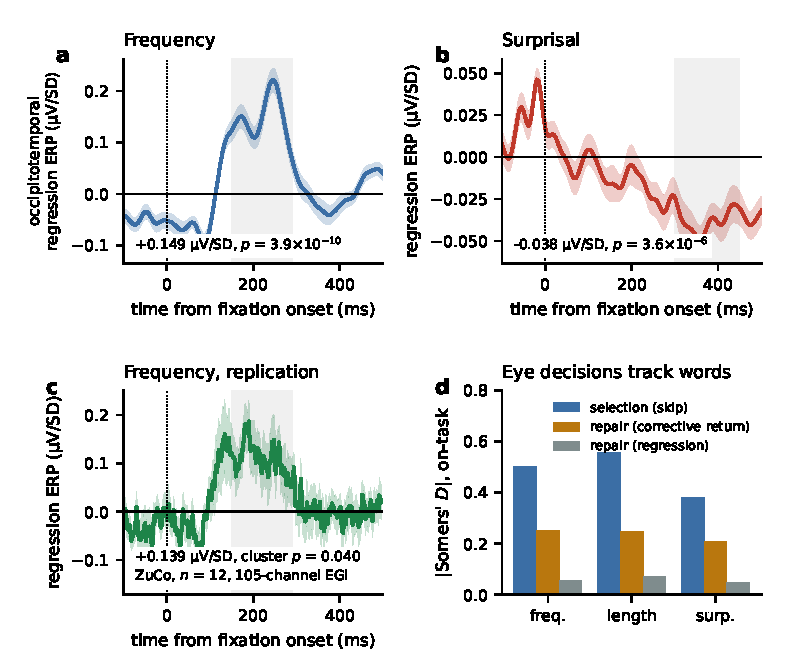
\includegraphics[width=0.78\textwidth]{fig2_instrument.pdf}
\caption{\textbf{The measures respond to word properties during engaged reading.}
(a) Overlap-corrected regression-ERP kernel for word frequency at occipitotemporal sensors.
(b) Kernel for contextual surprisal at centroparietal sensors. Shading is the standard error
across 44 readers; grey bands mark the a priori analysis windows. (c) The frequency kernel in
an independent 12-reader sample recorded with different hardware. (d) Rank-based association
between word properties and each of the three eye-movement decisions during on-task reading.}
\label{fig:instrument}
\end{figure}

\subsection{The reported spans behave like mind-wandering}

Because the primary sample uses retrospective span marking rather than probes, we checked that
the labels track the canonical behavioural signature before treating any null based on them as
informative. All 44 readers marked at least one span, per-reader rates ranged from 0.2\% to
24.2\% of fixations, and fixations inside a reported span were 5.0\% longer than the same
reader's on-task fixations (95\% CI $[3.3, 6.6]$, $p=7.9\times10^{-7}$, 39 of 44 readers). The
labels reproduce the effect that mindless reading is best known for.

\subsection{Mind-wandering leaves selection, repair and duration intact}

We then asked whether any of these sensitivities changed during reported mind-wandering
(Fig.~\ref{fig:preserved}). This is the first half of the dissociation, and it is a null we
treat as a quantity to be bounded rather than a test to be passed.

\paragraph{Selection.} A word counted as skipped only if the reader's scan path stepped over
it in a single forward saccade spanning at most four intervening words. Words lying inside larger positional gaps were excluded rather than scored. Those gaps are almost
entirely return sweeps between text lines (97\% of them, see below), and the words inside them are
passed over for reasons of display layout rather than of lexical access. This yielded 332{,}016 words, of which 21{,}633 fell inside a reported
mind-wandering span, from 36 readers with at least 150 words in each state. The influence of
word properties on skipping was unchanged. Retention of the on-task association was 100.5\%
for frequency (mind-wandering minus on-task $\Delta D=+0.0025$, 95\% CI $[-0.0167, +0.0214]$,
$p=0.80$), 101.8\% for length ($\Delta D=-0.0100$, $[-0.0283, +0.0099]$, $p=0.32$) and 103.1\%
for surprisal ($\Delta D=-0.0118$, $[-0.0326, +0.0099]$, $p=0.30$). Expressed relative to the
on-task effect, the frequency interval runs from $-3.3\%$ to $+4.2\%$. All three were
statistically equivalent within $\pm$10\% of the on-task effect
(TOST $p=1.1\times10^{-5}$, $2.6\times10^{-5}$ and $0.011$; BF$_{01}=5.4$, $3.5$ and $3.3$).
We set the smallest effect of interest from the literature rather than from these data.
\citet{reichle2010} report frequency and length effects that are essentially abolished before a
self-caught lapse, \citet{schad2012} report attenuations on the order of a third to a half at
their deeper level, and the instructed-goal contrast reported below attenuates the same slope by
34 to 44\%. A bound of 20\% is therefore already well inside the range the decoupling account
predicts, and 10\% is conservative by a further factor of two.

These nulls survived every control we ran. They were stable across skip-definition thresholds
from one to ten intervening words, unchanged when restricted to spans the reader marked as
fully off-task, present within each tertile of position through a run, and stable when any one
article was dropped. A relocation control, in which each reader's mind-wandering spans were
moved to random on-task positions of matched length and re-analysed 200 times, reproduced the
observed values ($p_{\text{perm}}=0.81$, $0.28$ and $0.31$), so even the small numerical
trends are not specific to mind-wandering. For context on sensitivity, the width of the
frequency interval means that an attenuation of the size the instructed-goal condition produces
below, roughly a third, would have been detected here with a very large margin.

\paragraph{Repair.} Refixation selectivity was retained at 96\% to 99\% (35 readers, all
$p>0.5$) and the tendency of regressions to target difficult words was retained at 74\% for
frequency ($p=0.25$), 73\% for length ($p=0.056$) and 100\% for surprisal ($p=0.99$; 38
readers). The length effect is the only hint of attenuation anywhere in the battery and it does
not survive correction across the three properties. Corrective-return selectivity could be
estimated in only 16 readers, because it requires enough single-skip events in both states
within a reader, and we therefore treat it as uninformative rather than as evidence either way.
The corrective-return \emph{rate}, which uses all 44 readers, is reported below.

\paragraph{Duration.} Across words, the mind-wandering slope was slightly larger than the
on-task slope, with signed retention of 114.6\% for frequency (paired $p=0.001$) and 111.6\%
for length (paired $p=0.007$). We do not interpret this as sharpened lexical control, for two
reasons. First, length is a visual property, and it was enhanced as much as frequency, which
is the signature of a global rescaling of log slopes rather than of anything lexically
specific. Second, the effect is not identified across words, because the words a reader
happens to encounter while mind-wandering are not a random sample. Since each corpus token was
read by up to 44 readers, and 7{,}264 of 10{,}183 tokens (71.3\%) were read both on-task and
during mind-wandering by different readers, mind-wandering status varies within token. A
two-way fixed-effects model absorbing token identity and reader identity, with reader-clustered
standard errors, roughly halved the estimate and removed its significance (frequency
$\beta=-0.0109$, SE $=0.0070$, $p=0.13$; surprisal $\beta=-0.0084$, $p=0.18$; length
$\beta=+0.0087$, $p=0.27$; $n=234{,}800$ word observations). The additive component was large
and highly reliable in the same model ($\beta=+0.103$, SE $=0.011$, $p=1.6\times10^{-11}$).
Mind-wandering moved the intercept, not the slope.

\paragraph{Brain.} The two neural channels differ sharply in what they can support, and we
separate them.

The occipitotemporal frequency response was preserved. In the overlap-corrected model the
frequency by mind-wandering interaction was $+0.024$\,\si{\micro\volt} ($p=0.30$, $n=44$),
which is $+16.0\%$ of the on-task effect with a 95\% interval of $[-12.5, +45.9]\%$. Because
the decoupling account predicts a reduction, the informative bound is one-sided: attenuations
greater than 8.2\% are excluded (BF$_{01}=3.6$). This response therefore behaves like the
behavioural measures.

The centroparietal surprisal response could not be tested usefully. The interaction was
$+0.005$\,\si{\micro\volt} ($p=0.79$), which is $-13.4\%$ of the on-task effect, but with a
95\% interval of $[-112.2, +81.6]\%$. The smallest change this design could have detected at
80\% power is 144\% of the on-task effect, so the test cannot distinguish a preserved N400 from
an abolished one. We report it as uninformative rather than as evidence of preservation. The
limit is the signal-to-noise ratio of the surprisal response itself, which is reliable at the
group level ($p=3.6\times10^{-6}$) but small in absolute terms ($-0.038$\,\si{\micro\volt} per
SD), so a 30\% modulation of it lies far below what 44 readers can resolve. A cluster-based
permutation test over the whole epoch and all sensors returned no cluster for either
interaction ($\min p=1.0$), which is consistent with both conclusions and decisive for neither.

The additive pattern seen in behaviour appeared in the neural data as well: a uniform
occipitotemporal amplitude offset of $+0.087$\,\si{\micro\volt} ($p=3.4\times10^{-5}$) with the
slope unchanged. Split-half reliability of the fixation-related potential was identical in the
two states when trial counts were matched (0.888 versus 0.889, $p=0.91$), so neither neural
result reflects noisier data during mind-wandering.

\begin{figure}[t]
\centering
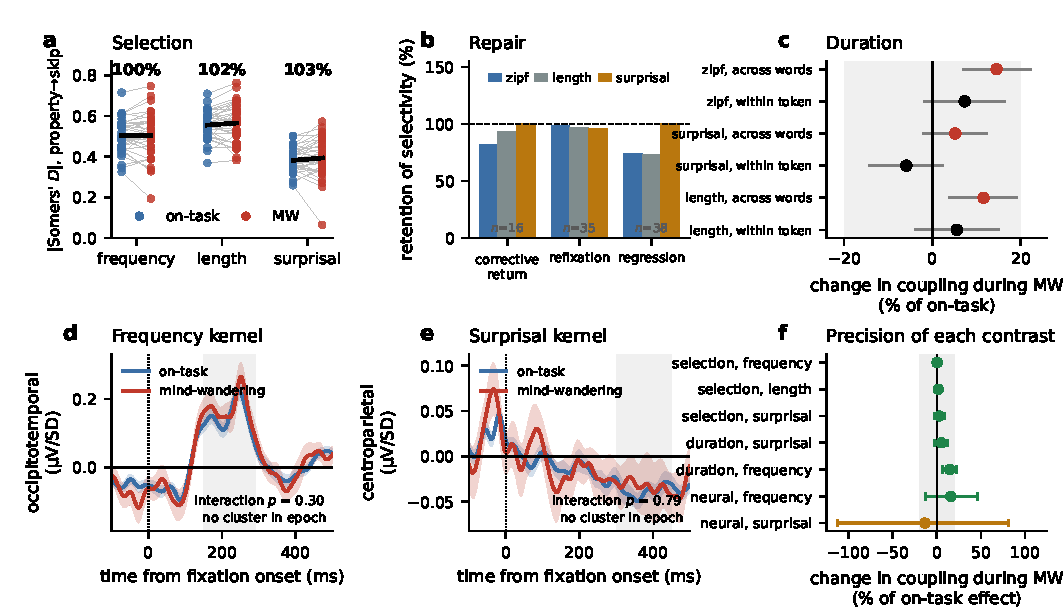
\includegraphics[width=\textwidth]{fig3_preserved.pdf}
\caption{\textbf{Mind-wandering spares word sensitivity at every level measured.}
(a) Rank-based association between word properties and skipping, per reader, on-task versus
mind-wandering; black lines join condition means, percentages give retention.
(b) Retention of selectivity for the three repair behaviours.
(c) Change in the fixation-duration slope, estimated across words (coloured) and within token
instance with reader and token fixed effects (black). Bars are 95\% intervals; the shaded band
is the $\pm$20\% equivalence region.
(d, e) Overlap-corrected kernels by state.
(f) Change in coupling for every contrast, with 95\% bootstrap intervals. Orange marks the
surprisal response, whose interval is too wide to constrain the question at all; the other
contrasts each exclude attenuations of more than a few percent.}
\label{fig:preserved}
\end{figure}

\begin{table}[t]
\centering
\small
\caption{Every coupling contrast, with what it can and cannot rule out. $\Delta$ is the change
during mind-wandering as a percentage of the on-task effect, positive meaning stronger coupling.
``Attenuation excluded'' is the one-sided 95\% bootstrap bound, that is, the smallest
reduction inconsistent with the data. The last column is the smallest change the contrast could have
detected at 80\% power. Neural rows use the overlap-corrected kernels from all 44 readers.}
\label{tab:equiv}
\begin{tabular}{llrrrr}
\toprule
Level & Predictor & Readers & $\Delta$ (\% of on-task) & Attenuation excluded & Detectable at 80\% \\
\midrule
Selection & frequency  & 36 & $+0.5$ $[-3.3, +4.2]$     & $>2.7\%$  & 6\% \\
Selection & length     & 36 & $+1.8$ $[-1.7, +5.2]$     & $>1.2\%$  & 5\% \\
Selection & surprisal  & 36 & $+3.1$ $[-2.7, +8.4]$     & $>1.7\%$  & 8\% \\
Duration  & surprisal  & 38 & $+5.2$ $[-2.0, +12.5]$    & $>0.9\%$  & 11\% \\
Duration  & frequency  & 38 & $+14.6$ $[+6.8, +22.4]$   & none      & 12\% \\
Neural    & frequency  & 44 & $+16.0$ $[-12.5, +45.9]$  & $>8.2\%$  & 43\% \\
Neural    & surprisal  & 44 & $-13.4$ $[-112.2, +81.6]$ & $>96.6\%$ & 144\% \\
\bottomrule
\end{tabular}
\end{table}

Table~\ref{tab:equiv} makes the asymmetry explicit. The three selection rows are the tightest
in the study: each excludes attenuations above a few percent and could have detected a change of
about 5 to 8\%. The duration rows are comparable, except that the frequency contrast is displaced
in the direction of stronger coupling, which the within-token model in
Fig.~\ref{fig:preserved}c attributes largely to which words readers happened to encounter. The
neural frequency row is looser but still useful, excluding attenuations above 8.2\%. The neural
surprisal row excludes nothing: it could not have detected the complete disappearance of the
effect, and no conclusion should be drawn from it in either direction.

\subsection{Reconciling this with the reported increase in skipping}

One result stands against the first half of the dissociation, and it is the most consistent
behavioural marker in the meta-analytic literature: readers skip more words when their minds
wander \citep{meziere2025}. Our data reproduce it, and then overturn it
(Fig.~\ref{fig:measurement}).

Scoring a word as skipped whenever it received no first-pass fixation anywhere in the reading
span gives a large effect in the expected direction: skipping rises from 0.439 to 0.648
($\Delta=+0.168$, 95\% CI $[0.131, 0.206]$, $p=7.4\times10^{-11}$, 41 of 44 readers).
Requiring instead that the scan path demonstrably stepped over the word reverses the sign.
With a threshold of at most four intervening words, skipping falls from 0.251 to 0.226
($\Delta=-0.042$, $[-0.057, -0.028]$, $p=1.8\times10^{-6}$, 38 of 44 readers). The reversal
holds at every threshold from one to ten.

The two definitions differ over words that lie inside large positional gaps in the scan path,
so what those gaps are matters. They are return sweeps. Clustering the bounding-box tops of the
stimulus words into text lines, steps spanning more than four words cross a line boundary in
96.6\% of on-task cases and 97.7\% of mind-wandering cases, against 4.5\% and 4.7\% of steps
between adjacent words (Fig.~\ref{fig:measurement}c). The words inside them are the last words
of one line and the first words of the next, which readers pass over for reasons of layout
rather than of lexical access, and which reading research conventionally treats separately. The
threshold is therefore not a free parameter; it recovers a category defined by the display.

Nor are the gaps periods in which gaze leaves the text. Within a page, the fraction of time not
spent on a mapped word was the same in the two states (0.166 versus 0.169, $p=0.49$), and the
interval between successive fixations was indistinguishable across states within every gap size
(medians of 26 to 43\,ms throughout). We note that the released derivative retains only fixations that could be mapped to a word. This
is therefore an argument from elapsed time rather than a direct observation of where gaze went. An
unobserved off-text fixation would have shown up as a long interval, and none does.

What differs between the states is structural. During mind-wandering 74\% of stepped-over words
lie inside large same-page forward jumps against 48\% on-task, while 29\% of on-task
stepped-over words come from page transitions against under 1\% during mind-wandering. Because
reported spans rarely straddle a page change, the naive measure is assembling the two states
from different kinds of gap.

\paragraph{The result does not depend on the exclusion.} Excluding words is a state-dependent
operation here, and the excluded words are not identical across states: relative to on-task, the
words excluded during mind-wandering were slightly more frequent ($\Delta=+0.16$ Zipf,
$p=1.7\times10^{-4}$), shorter ($\Delta=-0.29$ characters, $p=1.7\times10^{-6}$) and less
surprising ($\Delta=-0.35$ bits, $p=0.023$). We therefore repeated the primary analysis in two
ways that do not rely on the gap criterion. Using a purely layout-based rule, in which a word is
analysable if the reader fixated at least one word on the same text line both before and after
it, skipping still fell during mind-wandering (0.268 to 0.252, $\Delta=-0.035$,
$p=1.1\times10^{-5}$) and selectivity was still preserved (retention 96.9\%, 97.6\% and 99.1\%;
all $p>0.11$; Fig.~\ref{fig:measurement}e). Matching the exclusion rate across states within reader gave the same answer for selectivity
(99.4\%, 98.6\% and 101.0\%; all $p>0.4$). That procedure distorts the composition of the retained
set, so we do not read a rate contrast from it.

\subsection{Reading becomes more effortful, not more cursory}

The corrected picture of what mind-wandering does to the eyes is coherent and is the opposite
of skimming. Relative to on-task reading by the same readers, gaze durations were 14.6\%
longer (95\% CI $[10.3, 19.6]$, $p=2.2\times10^{-7}$, 40 of 44 readers), regressions were 18.1\%
more frequent
($p=1.3\times10^{-4}$, 39 of 44 readers), immediate refixations were 13.9\% more frequent
($p=0.006$, 34 of 44), corrective returns to skipped words were 12.6\% more frequent
($p=0.13$), and skipping was 18.5\% less frequent ($p=1.8\times10^{-6}$). Readers put more
work into each word and moved past fewer of them, while remaining exactly as sensitive to
which words deserved the work.

\begin{figure}[t]
\centering
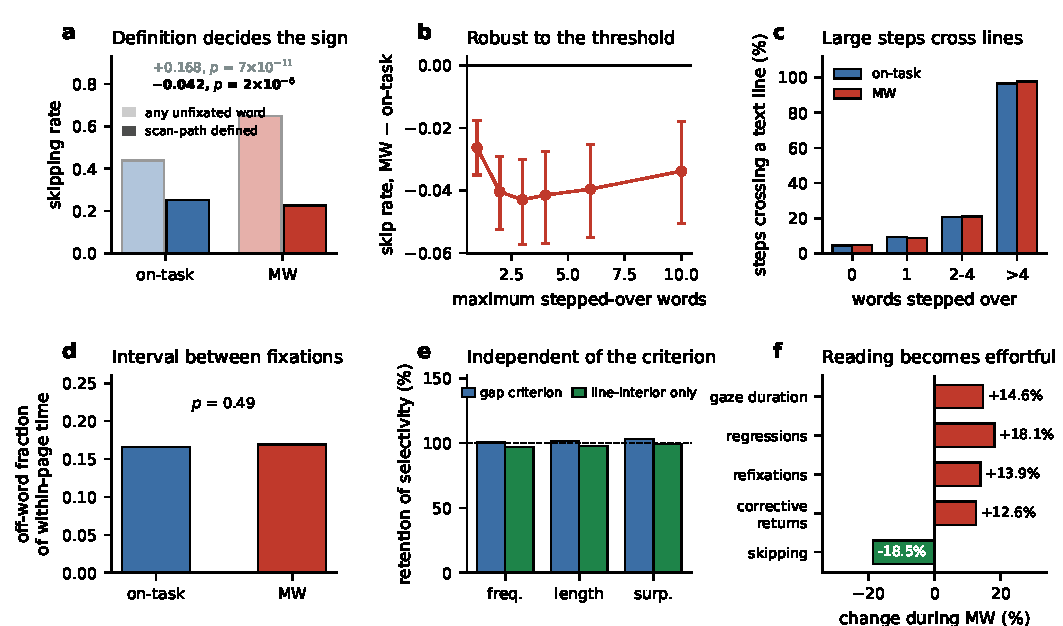
\includegraphics[width=0.78\textwidth]{fig4_measurement.pdf}
\caption{\textbf{The skipping marker depends on the definition, and the corrected profile
shows more effort rather than less.}
(a) Skipping rate under a naive definition (any unfixated word, pale) and a scan-path
definition (solid).
(b) The corrected effect across thresholds for the number of words a single forward saccade may
step over; bars are 95\% bootstrap intervals.
(c) Percentage of forward steps that cross a text line, by the number of words stepped over.
Steps larger than four words are return sweeps in both states.
(d) Fraction of within-page time not spent on a mapped word.
(e) Retention of skipping selectivity under the gap criterion and under a purely layout-based
criterion that uses only line-interior words.
(f) Change in each eye-movement measure during mind-wandering, computed within reader and
averaged.}
\label{fig:measurement}
\end{figure}

\subsection{Skimming and mind-wandering are different states}
\label{sec:goal}

If our measures were simply insensitive, they should also fail when coupling really does
change. They do not (Fig.~\ref{fig:states}).

In the independent sample, readers read the same kind of sentences either for comprehension or
while searching for a specific semantic relation. The instructed search made reading shallower
on every behavioural measure. Total reading time fell by 20\%, and readers fixated 30\% fewer
words. Coupling fell with it. The frequency slope on gaze duration dropped to 62.3\% of its
value in normal reading ($p=1.7\times10^{-4}$), and surprisal behaved identically (62.7\%,
$p=7.4\times10^{-5}$).

The neural response did not follow. The occipital frequency kernel changed by $+32.0\%$
($[-31.9, +88.1]\%$, $p=0.33$, $n=12$), and attenuations greater than 20\% are excluded, against
a behavioural attenuation of 34 to 44\%. With twelve readers this is a weak constraint, but it
is a constraint, and it points the same way as the frequency result in the primary sample.

This gives a three-way contrast that we think is the most informative comparison in the paper.
Under an instructed shallow goal, the brain continues to register each fixated word while the
eye-movement policy stops tracking word properties. Under spontaneous mind-wandering, neither
does. Skimming and mind-wandering are therefore not two points on a single axis of
disengagement. They are different states with different signatures. Skimming changes what the
eyes are being asked to do. Mind-wandering leaves that intact and changes something else.

Task and recording session are partly confounded in that dataset, because task order was fixed
for every reader. A third task split across both sessions separates the two influences: there is
a genuine session effect (frequency coupling at 84.9\%, $p=0.020$), but the task effect survives
within a single session, at 66.4\% for frequency ($p=0.002$) and 56.0\% for surprisal
($p=1.3\times10^{-4}$). Two further caveats, a predeclared lexical-versus-semantic dissociation
that was not supported and a scale artefact that understates both of our effects on the
conventional log scale, are reported in SI~S5 and SI~S6.

\begin{figure}[t]
\centering
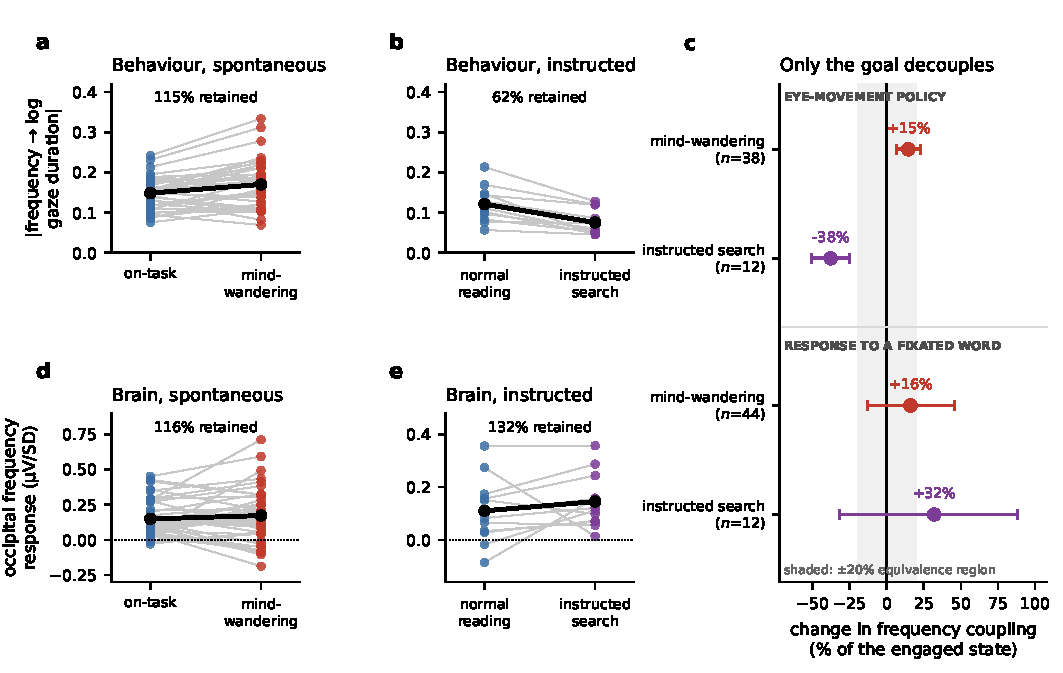
\includegraphics[width=\textwidth]{fig5_states.pdf}
\caption{\textbf{Skimming and mind-wandering are different states.}
(a, b) Frequency slope on log gaze duration, one point per reader, in the primary sample
(on-task versus mind-wandering) and in the independent sample (normal reading versus instructed
relation search). Black lines join condition means.
(d, e) The occipitotemporal frequency response over 150 to 290\,ms in the same four conditions,
one point per reader.
(c) All four cells on one axis, as the change in coupling expressed as a percentage of the
engaged state, with 95\% bootstrap intervals over readers. The point estimate is the mean
per-reader change divided by the group engaged-state effect, so a negative value is an
attenuation. Shading marks the $\pm$20\% equivalence region. The instructed goal attenuates the
eye-movement policy and leaves the brain response alone; mind-wandering does neither.
The neural interval in the instructed sample is wide, and excludes only attenuations greater
than about 20\%.}
\label{fig:states}
\end{figure}

\subsection{What changes is global state, not word-level processing}
\label{sec:state}

Mind-wandering is not invisible to these measures. What it changes is not specific to any
word. Four results establish that, and are reported in full in the Supplementary Information.

First, the fixation-related response does change in size, and only in size. Over 150 to
290\,ms the mind-wandering minus on-task field is reliable and is strongly anticorrelated with
the ordinary fixation field ($r=-0.872$): it is a scaled copy of it. A single proportional
factor of 25.8\%, fitted leave-one-reader-out, accounts for 76.1\% of the group map and leaves
no reliable residual ($p=0.277$). A change of that kind applies equally to every word, so it
cannot carry information about which word was processed less, in the way a change in the
frequency or surprisal kernel would (SI~S1, Fig.~\ref{fig:gain}).

Second, the extra effort is not aimed anywhere. The mind-wandering increase in fixation
duration, regressions and refixations was flat across quartiles of word difficulty (trends
$p\geq0.25$), and the contribution of extended context to reading time and to the N400 was
unchanged ($p=0.37$ and $p=0.28$). Readers are not selectively going back over the words that
gave them trouble. Only regressions accumulate: the rate climbs steadily through an episode
($+0.022$ per additional two seconds, $p=0.0012$), which 300 matched on-task stretches never
reproduce (SI~S2).

Third, slow state markers move. Pupil diameter rose ($+0.20$\,z, $p=1.5\times10^{-4}$) and
central beta power fell ($-0.074$\,z, $p=2.4\times10^{-4}$) at the onset of a reported span,
neither at position-matched control onsets. Readers also became less like one another, but only
in the component that word properties do not explain: overall inter-subject alignment barely
moved (97.1\% retention, $p=0.30$), while alignment in the residual after regressing out
frequency, length and surprisal fell to 86.7\% ($p=0.037$, permutation $p=0.007$)
(SI~S3, Fig.~\ref{fig:changes}).

Fourth, a continuous index of how strongly the text is currently driving a reader, built without
any reference to the reports, does not detect mind-wandering (AUC $0.506$, $p=0.18$), while an
index of how hard the reader is working does ($0.528$, $p<10^{-4}$). Detectors that appear to
measure attention to text are measuring effort and arousal (SI~S4, Fig.~\ref{fig:index}).

\subsection{Comprehension fails where the mind was, not where the eyes were}
\label{sec:comp}

Word processing is preserved, but comprehension is not. This is the second half of the
dissociation, and it is where the consequence of a lapse becomes visible. The released dataset
includes one multiple-choice question per page, which gives an outcome that is independent of the
physiology. It provides the first test of the reports against something other than another
measure of the reader's body (Fig.~\ref{fig:comp}).

At page level the reports behave as they should. Accuracy fell from 0.673 to 0.552 on pages with
a reported span. In the tightest specification, which holds reader and story constant, the cost
is 5.9 accuracy points ($p=0.006$), a within-cell permutation gives $p=0.014$, and the effect is
graded with the amount of the page covered ($p=7.2\times10^{-4}$). It is specific to the page
whose question is asked rather than to the rest of the story.

The more informative question is where on the page it matters. A large language model read each
page against its question and marked the answer-bearing sentences, a median of 21\% of the page.
Two checks say the spans are real. A second language model scoring from those sentences alone
recovers the gold answer at 0.859, against 0.848 from the whole page, so the spans carry the
answers. A separate annotation of the same items, built automatically from question-to-sentence
overlap, agrees with them exactly on 32 of 50 and at a mean overlap of 0.825.

Mind-wandering on the answer span cost $-0.073$ in accuracy (95\% CI $[-0.092, -0.053]$,
$p=1.7\times10^{-13}$), with reader and item held constant. Mind-wandering elsewhere on the same
page cost $-0.035$ and was not reliable ($p=0.064$). Accuracy runs 0.680 with no lapse anywhere,
0.640 with a lapse on the page but not on the answer, and 0.405 with a lapse on the answer
itself.

\begin{figure}[!t]
\centering
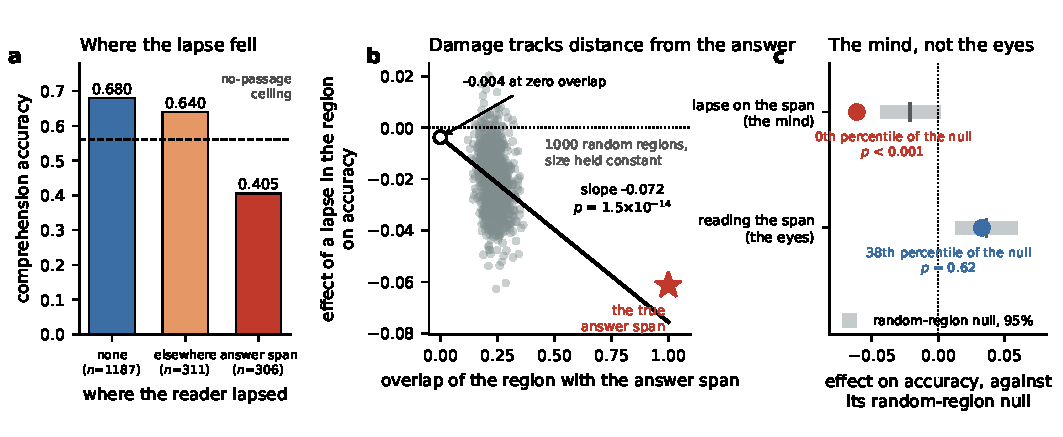
\includegraphics[width=\textwidth]{fig9_comprehension.pdf}
\caption{\textbf{Comprehension fails where the mind was, not where the eyes were.}
(a) Raw accuracy by where the reported lapse fell, with the no-passage answerability ceiling
marked. These are unadjusted proportions; the modelled effect holding reader and item constant
is smaller.
(b) The effect of a lapse on accuracy for each of 1000 randomly placed regions of the same size
on the same page, against how much each region overlaps the annotated answer span. Region size
is held constant, so only location varies. The open circle is the fitted value at zero overlap
and the star is the true answer span.
(c) The same comparison run twice. Where the mind was, at which specific words, is more extreme
than all 1000 random regions. Where the eyes went sits inside the null. Bars are the
random-region null intervals: the mind's from the stored 2.5th, 50th and 97.5th percentiles of
its 1000 regions, the eyes' as mean $\pm 1.96$ standard deviations, which is the only summary
of that null that was retained.}
\label{fig:comp}
\end{figure}

Two controls carry this result. First, we repeated the analysis on 1000 randomly placed regions
of the same size on the same page. The observed effect is more extreme than all 1000, and a
size-matched control region gives essentially nothing ($-0.0017$). Second, and more useful,
the effect across those random regions scales linearly with how much each one overlaps the true
answer span (slope $-0.072$, $p=1.5\times10^{-14}$), and falls to $-0.004$ at zero overlap.
Region size is held constant, so the only thing varying is location. Damage tracks distance from
the answer. The effect also survives adding coverage, fixation count and dwell time on the span
($-0.053$, $p=4.6\times10^{-6}$), so it is not simply that those readers did not read it.

That a reader misses what they were not attending to is not surprising on its own. The
informative part is that the same reasoning fails when applied to the eyes. Reading the answer
span more does predict accuracy at first glance ($+0.033$, $p=0.016$). A size-matched control
region predicts it just as well ($+0.025$, difference $p=0.65$). Against the random-region
distribution the true answer span sits at the 38th percentile ($p=0.62$). An
independent set of span annotations reproduced this null at the 39th percentile. Where the mind
was, at which specific words, is decisive. Where the eyes went is unremarkable.

The damage is also unflagged. A lapse on the answer span produced wrong answers ($-0.061$,
$p=4\times10^{-8}$) rather than expressions of uncertainty, which rose only marginally
($+0.021$, $p=0.099$). Readers do not appear to know what they have lost.

We report the size of this effect in proportion. Adjusting for reader, item, reading amount and
mind-wandering elsewhere, eliminating lapses on answer spans would raise accuracy by 1.79 points
(95\% CI $[0.80, 2.85]$), which is 4.9\% of all errors (95\% CI $[2.2, 7.7]$). The effect is
large where it lands and modest in aggregate, because only 17.5\% of trials carry a lapse on the
answer span. The raw contrast between 0.680 and 0.405 overstates the population effect
considerably.

This section carries a caveat that we would rather state than bury. The item bank was designed
to encourage attentive reading rather than to measure it, and a language model with no passage
at all answers 56\% of the items correctly. The reading-dependent range is therefore narrower
than the raw accuracies suggest. Because the localisation effect is identified within item, item
answerability is absorbed and cannot drive it, but the absolute sizes should be read with the
ceiling in mind.

\section{Discussion}

The reader whose mind has wandered is still reading the words. What has stopped is the making of
anything out of them.
Across three levels of eye-movement control we could not detect any reduction in word
sensitivity during self-reported mind-wandering, and the same held for the lexical component of
the fixation-locked brain response. The
strongest of these nulls is the one that matters most for the decoupling account. Whether a
word is skipped is decided on parafoveal information before the word is fixated, and it is the
decision the meta-analytic literature identifies as the most consistent behavioural marker of
mindless reading \citep{meziere2025}. In our data the lexical control of that decision was
statistically equivalent to its on-task value within $\pm$10\%, several times tighter than the
attenuations the decoupling account predicts and than the one our own instructed-goal condition
produced.

We take the positive control seriously. An instructed shallow goal attenuated the same
frequency slope by a third within a single session. Readers who are told to search a sentence
for a specific relation stop letting word difficulty govern how long they look. So the
measures are capable of registering a change in coupling, and their failure to register one
during mind-wandering is evidence rather than absence of evidence.

Why, then, has the field converged on the opposite conclusion? Part of the answer is likely
the measurement issue we document. In continuous multi-page reading, scoring any unfixated
word as skipped conflates a saccade that steps over a word with a gap in the correspondence
between gaze and text. The two are not equally distributed across states, and the resulting
bias is large enough to invert the sign of the effect. We do not claim that this artefact is present in prior work, and we are not in a position to know.
The operational definition of skipping is frequently not reported in enough detail to tell. Much
of the contributing literature also used isolated sentences, where the scan path is short and gaze
is easier to keep in register with the text. The point is narrower
and, we think, more useful. The marker is definition-sensitive in continuous reading, the two
definitions can differ in sign, and the diagnostic that separates them is cheap to run.

A second part of the answer may be paradigm. \citet{reichle2010} used self-caught reports
during sentence-by-sentence reading of a novel, and analysed the intervals leading up to a
report. Our spans are retrospective, and their onsets are correspondingly imprecise. It is
possible that a brief decoupled interval exists immediately before a reader notices the lapse,
and that our labels smear across it. That is a real limitation, but it cuts both ways. It
means our estimate is a property of sustained mind-wandering as readers themselves demarcate
it, which is the state that matters for the everyday experience the phenomenon is named after.

The positive results point somewhere different from gating. Mind-wandering made reading more
effortful. Readers looked longer, went back more often, refixated more often, and skipped less,
all while remaining exactly as sensitive to which words merited that treatment. This is hard to
reconcile with an account in which the perceptual stream is attenuated.

It is also hard to reconcile with the obvious alternative, that readers are repairing words they
failed to process. Repair should be aimed at difficult words, and none of the three effort
measures was. A direct test of whether extended context still contributes to reading time and to
the N400 was likewise null. Readers are not selectively going back over the words that gave them
trouble.
Nor is all of the extra effort the same kind of thing. Longer fixations and refixations appear immediately at the start of an episode and stay flat, which is what a change of state looks like. Regressions instead climb steadily for as long as the episode lasts, and do so specifically during reported spans. Something accumulates, it expresses itself as undirected backtracking, and it is indifferent to which words are hard.

Two positive results tell us where to look for the failure. The first is the loss of alignment
across readers. Word-level coupling is low-dimensional. A reader can remain perfectly sensitive
to frequency and surprisal while constructing something quite different from the text, and the
inter-subject measure is sensitive to that residual in a way that word-level regression is not
\citep{simony2016,nastase2019}. The second is the comprehension result. Mind-wandering predicts
failure on the question for that page, and the cost is concentrated on the specific sentences
that carry the answer rather than spread across the page. Both point the same way. What fails
is not the identification of words but what is built from them.

The comprehension analysis also sharpens the main claim in a way the coupling results alone
cannot. If word processing is intact, one might expect gaze on the answer-bearing sentences to
predict whether the answer was retrieved. It does not, once a size-matched control region and a
random-region distribution are taken into account. The subjective report of where attention was
carries content-specific information that the objective record of where the eyes went does not.
That asymmetry is difficult to reconcile with an account in which mind-wandering works by
withdrawing the eyes from the words.

Taken with the finding that inter-reader alignment falls only in the component that word
properties do not explain, the account we would put forward is that the reader loses the thread
rather than the words. Word identification continues and the eyes keep responding to it. What degrades is the higher-order representation that makes one word follow from the last. Its
behavioural expression is a reader who goes back more and more as the episode runs on, without
knowing quite where to go back to. We stress that this is the account our data are consistent with rather than one they establish. What the data localise is the level at which reading fails: downstream of word identification and of the eye-movement policies that word identification drives. We cannot say which downstream process fails. Integration into a situation model, its maintenance
in working memory, and the selection that keeps it updated are all candidates, and this design
does not separate them. The two measures that would test it directly,
the N400 and the contribution of extended context, are respectively unmeasurable here and null. The state changes we observed, a pupil dilation
and a cortical desynchronisation time-locked to onset and absent at matched control onsets,
are consistent with that reading, though neither is diagnostic of a specific mechanism on its
own \citep{smallwood2011pupil,kam2011,braboszcz2011}.

The rescaling result offers an account of one of the more puzzling features of this literature.
Mind-wandering has a real neural signature, and yet fixation-locked activity carries very little
information about what a reader took from the text. A proportional reduction in the response to
every word explains both facts at once. It is detectable, because the overall amplitude drops.
It is uninformative about content, because it drops equally for every word. A change in the
frequency or surprisal kernel would have been informative in that way, and there is no such
change.

The neural side of this study is asymmetric and we would not want that glossed over. The
frequency response is measured well enough to constrain the question: an attenuation of more
than 8.2\% is excluded, which is tighter than the effect an instructed goal produces. The
surprisal response is not. Its amplitude is small enough relative to trial noise that 44 readers
and 400,000 fixations cannot detect even its complete abolition, so the semantic channel remains
open. Closing it will need either a paradigm that produces a larger N400, such as strongly
constraining sentence contexts, or a great deal more data per reader. We say this plainly
because a reader skimming the figures could otherwise take the two neural rows to carry equal
weight, and they do not.

Two further limitations deserve statement. The mind-wandering and instructed-goal comparisons
come from different samples, so the contrast between them generalises across laboratories but
does not identify the goal as the causal switch. And the corrected skipping analysis conditions on the reader having scanned the local region.
That is a state-dependent selection, and although the conclusion survived a layout-based rule
and an exclusion-matched analysis, no version of this measurement is free of the choice
entirely.

\paragraph{What is established and what is inferred.} The levels of this argument are not
equally supported, and the vocabulary this literature uses for them is loose enough that they
can be run together. We separate them explicitly. Word identification and the sensitivity of eye-movement policy to word properties are preserved,
and preserved with stated bounds. Those bounds are $\pm$10\% on selection and 8.2\% on the
occipitotemporal frequency response, and an instructed goal produces a larger attenuation than
either admits. That is the established part.
Contextual integration is unresolved in either direction; the N400 test here is uninformative,
and the behavioural evidence bearing on it is indirect. Global state clearly changes: pupil
dilation, cortical desynchronisation, and a proportional reduction of the fixation response.
Comprehension clearly fails, and fails on the specific content the reader was absent for. The
step from those facts to a failure in constructing and maintaining a passage-level
representation is an inference we think is the most plausible available, not a measurement.
Nothing here shows that attention never decouples from perception, and neural work outside
reading gives good reason to think it sometimes does. What these data exclude is narrower and more useful. In the specific, testable form that predicts
weakened lexical control of the eyes and of the fixation-locked response, the decoupling account
does not describe sustained, self-demarcated mind-wandering in continuous reading. The failure lies downstream of word
identification.

For applied work the implication is direct. Some systems infer attentional state from how the eyes respond to text, in tutoring software, in
reading assessment, or in driver monitoring. Our data suggest that this signal is not diagnostic
of spontaneous mind-wandering, whatever else it may track. In this dataset it tracked task set. A reader who has been told to skim and a
reader whose mind has wandered produce opposite changes in word-level coupling, and confusing
them will produce detectors that work in the laboratory and fail in the field.

The continuous index makes the same point in a form that is easy to test elsewhere. An index of
how strongly the text is currently driving a reader, built without reference to any report, is
at chance for mind-wandering, while an index of how hard the reader is currently working is not.
Detectors that appear to measure attention to text are measuring effort and arousal. That may
still be useful, but it is a different quantity, and the distinction matters as soon as a system
is asked to decide whether a reader has understood something rather than whether they are
tired.

\section*{Acknowledgements}

[To be completed.]

\section*{Author contributions}

[To be completed.]

\section*{Competing interests}

The authors declare no competing interests.

\section*{Data and code availability}

The primary dataset is openly available \citep{roammdata} and the control dataset is distributed
by its authors \citep{hollenstein2018}. Analysis code, the preregistration documents, and the
derived tables needed to reproduce every figure are available at [repository].

\bibliography{refs}

\clearpage
\setcounter{figure}{0}
\renewcommand{\thefigure}{S\arabic{figure}}
\section*{Supplementary Information}

These analyses are reported in full here rather than in the main text because each
supports the argument without being part of its spine. Sections S1 to S4 describe what
does change during mind-wandering, summarised in Section~\ref{sec:state}. Sections S5 to
S7 concern the control sample. Sections S8 and S9 record two reliable but peripheral
observations.

\subsection*{S1. The fixation response rescales rather than reconfigures}

If word processing is preserved, the brain response to a fixated word should still differ
between states in some way, because fixation-related potential amplitude does shift. The
question is what kind of difference it is. A response can change in two ways. Its pattern can
change, meaning different sensors are involved or the timing differs, which would point to a
different configuration of underlying sources. Or the same pattern can simply get smaller,
which would point to the same processing at lower gain.

These predict different things about the difference map. If the pattern changes, the difference
between states should have a shape of its own. If only the size changes, the difference should
look like a scaled copy of the ordinary response (Fig.~\ref{fig:gain}).

It looks like a scaled copy. Over 150 to 290\,ms the mind-wandering minus on-task field is
reliable (global field power $0.067$\,\si{\micro\volt}, sign-flip $p=2.0\times10^{-4}$) and is
strongly anticorrelated with the on-task fixation field itself ($r=-0.872$, bootstrap 95\% CI
$[-0.931, -0.605]$). Estimating a single proportional scaling factor with a leave-one-reader-out
fit gives an attenuation of 25.8\% (95\% CI $[13.8, 39.7]$), which accounts for 76.1\% of the
variance in the group map. After subtracting that rescaling, no reliable residual field remains
($0.032$\,\si{\micro\volt}, $p=0.277$). The effect occupies 172 to 266\,ms (familywise cluster
$p=0.0056$).

One number therefore describes the whole neural effect of mind-wandering on the response to a
fixated word. The response keeps its shape and loses about a quarter of its size. An earlier
analysis of these data, which retained polarity when comparing topographies, appeared to show a
novel scalp configuration. That was a property of the test rather than of the data, and the
rescaling analysis resolves it.

This is why the main text treats the neural change as a change of state. A proportional change
in amplitude applies equally to every word. It cannot carry information about which particular word was processed less, in the way a
change in the frequency or surprisal kernel would. The neural signature of mind-wandering is
real, and it is uninformative about content by construction.

These are sensor-level results. We do not interpret the scalp map as source localisation.

\begin{figure}[t]
\centering
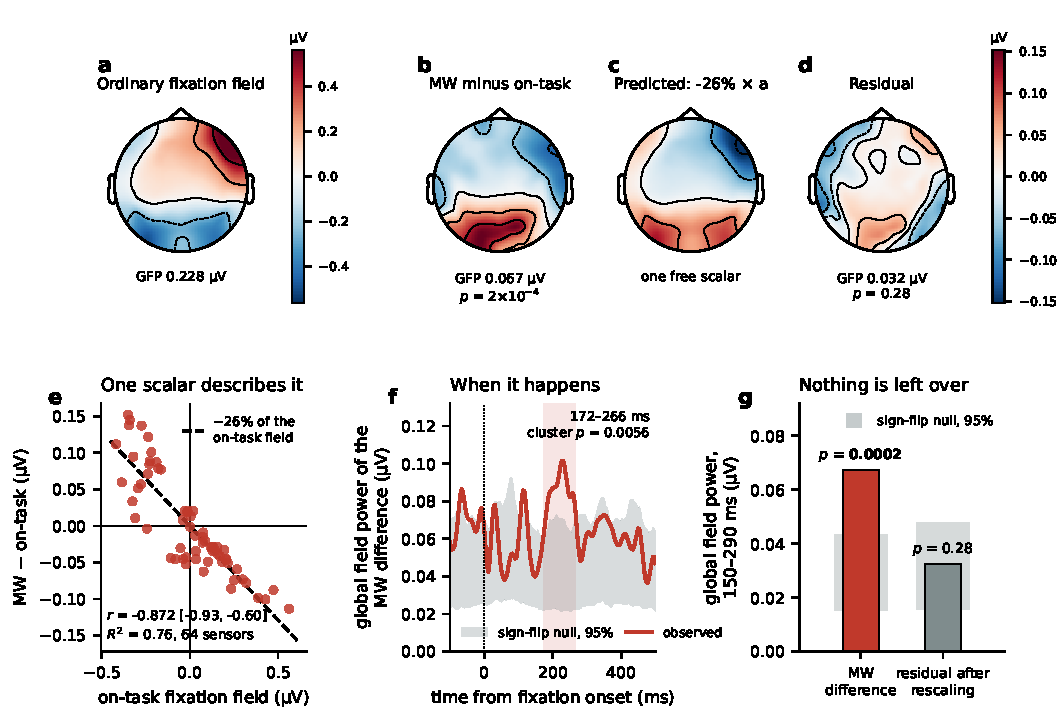
\includegraphics[width=\textwidth]{fig6_gain.pdf}
\caption{\textbf{Mind-wandering rescales the fixation response rather than reconfiguring it.}
(a) The overlap-corrected response to a fixated word on task, averaged over 150 to 290\,ms,
as a scalp field.
(b) The mind-wandering minus on-task difference field over the same window, on its own colour
scale.
(c) What a single proportional scaling of panel a predicts, using the leave-one-reader-out
factor of $-25.8$\%. One free parameter.
(d) What is left after subtracting that prediction.
(e) The same relationship channel by channel. Each point is one of the 64 sensors; the dashed
line is the fitted proportional model.
(f) Global field power of the difference field through the epoch, against a sign-flip null over
readers. Shading marks the familywise-corrected cluster.
(g) Global field power in the analysis window before and after the rescaling, each against its
own sign-flip null. Panels are sensor-level and are not interpreted as source localisation.}
\label{fig:gain}
\end{figure}

\subsection*{S2. The extra effort is undirected, and one part of it accumulates}

If the extra looking were repair, it should be aimed at the words that need repairing. It is
not. Splitting words into quartiles of contextual surprisal within each reader, the
mind-wandering increase was flat across quartiles for fixation duration (trend $p=0.25$),
regressions ($p=0.33$) and refixations ($p=0.54$). The same holds for the one direct test of
extended-context integration we can run: comparing surprisal computed over the whole preceding
passage against surprisal computed within the sentence alone, the contribution of extended
context to reading time and to the N400 was unchanged during mind-wandering ($p=0.37$ and
$p=0.28$). Whatever is failing, it is not showing up as a selective loss of context-based
prediction.

The three effort measures do, however, behave differently over time. Fixation duration and
refixation are step changes: fully present in the first two seconds of an episode and flat
thereafter (trends $p=0.63$ and $p=0.49$; against matched on-task stretches, $p_{\text{perm}}
=0.52$ and $0.43$). Regressions are not. The regression rate rises steadily through an episode,
from $+0.016$ above the reader's own baseline in the first two seconds to $+0.080$ after ten
seconds (linear trend $+0.022$, 95\% CI $[0.011, 0.034]$, $p=0.0012$, 26 of 37 readers). This
is specific to reported spans: 300 matched on-task stretches of the same length distribution
never produced a trend this large ($p_{\text{perm}}<0.005$), and it survives removing each
reader's position through the run ($+0.022$, $p=0.0007$), so it is not time on task.

Something therefore accumulates across a mind-wandering episode, and what it produces is
backtracking rather than slower or more repetitive fixating. It does not accumulate in a way
that tracks word difficulty.

\subsection*{S3. Slow state changes and inter-subject alignment}

Two things changed reliably (Fig.~\ref{fig:changes}a--c). Time-locked to the onset of a
reported span, pupil diameter increased ($+0.20$\,z, $p=1.5\times10^{-4}$) and central beta
power decreased ($-0.074$\,z, $p=2.4\times10^{-4}$), neither of which appeared at
position-matched control onsets drawn from on-task reading. This is a slow change in global
state, and it is the natural counterpart of the additive shifts in fixation duration and
fixation-related potential amplitude reported in the main text.

Second, readers became less like each other, and it is worth being precise about which part of
them. Using a leave-one-reader-out template built from other readers' on-task gaze durations for
the same word, overall alignment barely moved (retention 97.1\%, $p=0.30$), and removing the
additive and scale shift by z-scoring within state changed nothing (97.0\%, $p=0.29$). Most of
what readers share is driven by word properties, and that component is preserved, exactly as
the coupling analyses in the main text would predict. Removing it is what exposes the effect. In the residual
after regressing out frequency, length and surprisal, alignment fell from 0.201 to 0.175
(retention 86.7\%, $\Delta=-0.027$, 95\% CI $[-0.051, -0.002]$, $p=0.037$), and shuffling the
mind-wandering labels within reader at matched count never reproduced it
($p_{\text{perm}}=0.007$). The earlier report of a drop in raw gaze inter-subject correlation in
these data ($\Delta=-0.028$, $p=0.025$) is consistent with this once the difference in template
construction is taken into account.

So the loss of alignment is confined to the part of gaze behaviour that word properties do not
explain. Readers keep responding to the same words in the same way. What diverges is everything
else.

\begin{figure}[t]
\centering
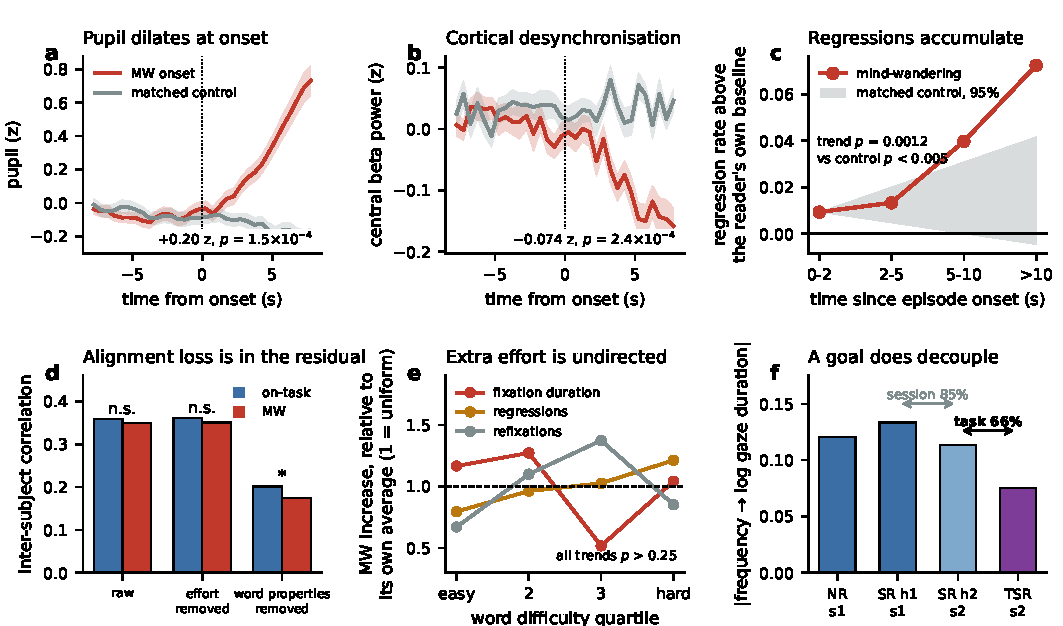
\includegraphics[width=0.78\textwidth]{fig8_changes.pdf}
\caption{\textbf{What changes during mind-wandering, and the positive control.}
(a, b) Pupil diameter and central beta power time-locked to the onset of a reported span,
against position-matched control onsets. Shading is the standard error across readers.
(c) Regression rate through an episode, relative to each reader's own on-task baseline. The band
is the 95\% range of trends from 300 matched on-task stretches of the same length distribution.
(d) Inter-subject alignment against a leave-one-reader-out template, before and after removing
the additive shift and the word-property component.
(e) The mind-wandering increase in each effort measure across quartiles of word difficulty,
scaled to its own average. A flat line means the increase is uniform.
(f) Frequency coupling in the independent sample by condition, showing the session effect
between the two halves of the sentiment task and the task effect within the second session.}
\label{fig:changes}
\end{figure}

\subsection*{S4. A continuous index of text-driven reading does not move}

Every automatic measure of mind-wandering we are aware of is trained on mind-wandering reports.
Asking whether such a measure captures attention is therefore circular, because it captures
whatever the reports capture. We built an index that is never shown the reports, and asked what
it does (Fig.~\ref{fig:index}).

The logic is the first principle the paper started from. If a reader is attending to the text,
properties of the words should be governing behaviour. We fit that relationship on on-task
fixations only, predicting log fixation duration from frequency, length and surprisal with
reader effects (Zipf $-0.0128$, length $-0.0014$, surprisal $+0.0028$). Every fixation then has
a duration that the text alone predicts. In a rolling window of 25 fixations we regressed
observed duration on predicted duration, with both centred inside the window. The centring is
what makes the index specific. It removes any overall speeding or slowing, and leaves only the
question of whether harder and rarer words are currently getting proportionally longer looks.
We scored the result as a within-reader percentile, so the index runs from 0 to 100.

The index does not distinguish mind-wandering from on-task reading. Its mean is 50.1 on task and
48.4 during reported spans, a difference of $-1.6$ points (95\% CI $[-4.3, +0.7]$, $p=0.18$),
with 24 of 44 readers in the predicted direction, which is chance. As a classifier of individual
fixations it reaches an area under the curve of 0.506.

The same pipeline applied to a level-based index behaves differently. Taking the within-reader
percentile of raw fixation duration, that index rises from 49.8 on task to 52.8 during reported
spans ($+3.1$ points, 95\% CI $[+2.1, +4.0]$, $p<10^{-4}$, area under the curve 0.528).

The two indices differ in one respect. One tracks the slope relating word properties to
behaviour. The other tracks the level of behaviour. Mind-wandering moves the level and leaves
the slope alone. This is the same conclusion as the rest of the paper, expressed as a signal
that runs continuously through a reading session rather than as a set of interaction terms.

\begin{figure}[t]
\centering
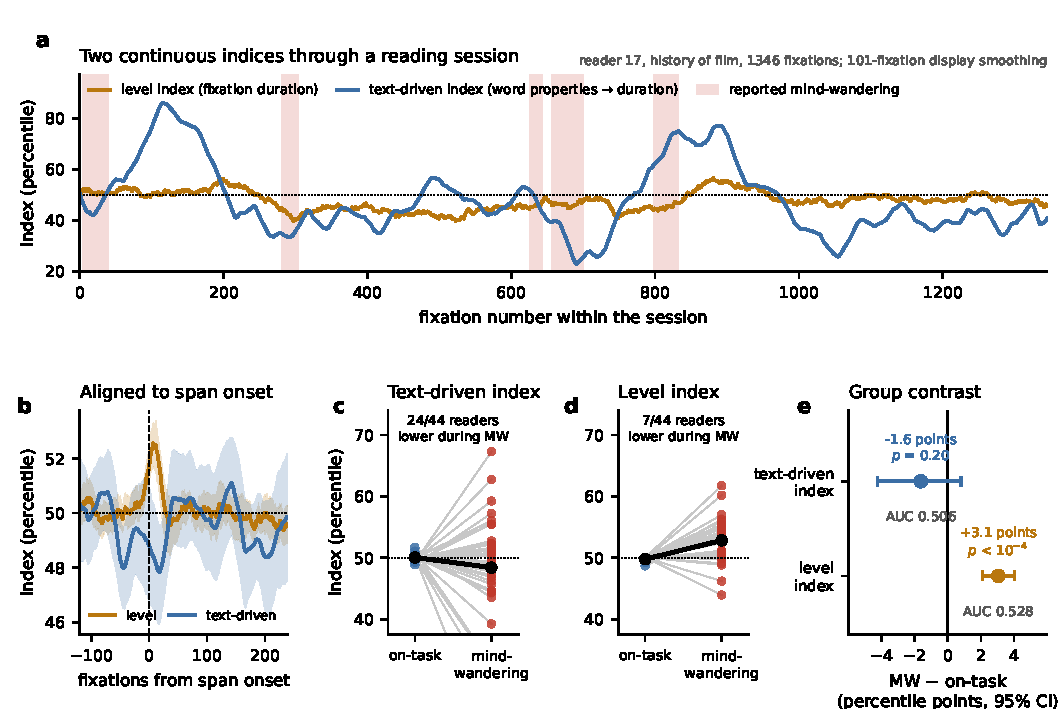
\includegraphics[width=\textwidth]{fig7_index.pdf}
\caption{\textbf{A continuous index of text-driven reading does not move; a level index does.}
(a) Both indices through one reader's session. The text-driven index is the rolling slope of
observed on text-predicted log fixation duration, centred within the window; the level index is
the within-reader percentile of raw fixation duration. Shading marks reported mind-wandering.
The session is the one whose two state contrasts fall closest to the group means among sessions
with at least five reported spans, and the traces are smoothed over 101 fixations for display
only.
(b) The same two indices aligned to the onset of a reported span, averaged within reader and
then across readers, with 95\% bootstrap bands. Descriptive; the tests are in (c) to (e).
(c, d) Each reader's mean index by state.
(e) The state contrast for both indices, with 95\% bootstrap intervals over readers, and the
area under the curve for classifying individual fixations. The index that never sees a
mind-wandering report is at chance.}
\label{fig:index}
\end{figure}

\subsection*{S5. The predeclared lexical-versus-semantic dissociation}

A predeclared test for a selective dissociation between lexical and semantic attenuation under
the shallow goal was not supported, and we do not report one. The apparent effect was an
artefact of collinearity between the two predictors, and the bivariate estimates attenuate
about equally.

\subsection*{S6. A scale artefact in how coupling is reported}

We also note a scale artefact that runs through this literature. When coupling is expressed as
a slope on log duration, a purely additive change in duration rescales the slope by the change
in the mean. Mind-wandering slows reading by 16\%, so an unchanged coupling would appear as
86.2\% retention on the log scale; instructed search speeds reading by 11\%, so an unchanged
coupling would appear as 112.0\%. Both of our effects are therefore understated on the scale
on which they are conventionally reported. On the raw millisecond scale, mind-wandering
retention is 133.8\% and instructed-search retention is 53.4\%.

\subsection*{S7. Session and materials in the control sample}

The contrast is also partly confounded with recording session, because the task order in that
dataset was fixed for every reader and the two tasks fell in different sessions
\citep{hollenstein2018}. A third task, sentiment reading, was split across both sessions, and
splitting it at its midpoint separates the two influences. There is a genuine session effect:
frequency coupling fell to 84.9\% between the first and second half of the sentiment task
($p=0.020$), with task and materials held constant. The task effect nevertheless survives
within a single session, at 66.4\% for frequency ($p=0.002$) and 56.0\% for surprisal
($p=1.3\times10^{-4}$). The same decomposition shows that materials are not neutral: reading
film-review sentences produced stronger coupling than reading encyclopedic sentences (110.5\%
for frequency, 134.2\% for surprisal). A comparison of the two deep tasks pooled across sessions
therefore averages a materials effect against a session effect of the opposite sign, and cannot
be read as evidence that materials are irrelevant. The split assumes that sentence index
corresponds to presentation order, which the dataset documentation supports but which we could
not verify directly.

\subsection*{S8. Onset intervals}

The fixation step at the start of a reported span was followed by
an interval longer than 500\,ms in 6.8\% of cases, against 0.6\% of steps taken within a state.
The enrichment is elevenfold. Because span onsets are marked retrospectively, we cannot tell
whether these long intervals precipitate the lapse, coincide with it, or are what makes a
reader remember where the lapse began, and we draw no inference from them.

\subsection*{S9. Materials and coupling}

In the control sample, frequency and surprisal coupling were
stronger for film-review sentences than for encyclopedic sentences (110.5\% and 134.2\%
respectively, within the first session). We report this because it bears on how the
deep-reading conditions of that dataset should be compared, not because we can explain it.


\end{document}
